% Options for packages loaded elsewhere
\PassOptionsToPackage{unicode,linktoc=all,pdfwindowui,pdfpagemode=FullScreen}{hyperref}
\PassOptionsToPackage{hyphens}{url}
\PassOptionsToPackage{dvipsnames,svgnames*,x11names*}{xcolor}
%
\documentclass[
  cn,11pt,chinese,bibstyle=apalike]{elegantbook}
\usepackage{lmodern}
\usepackage{amssymb,amsmath}
\usepackage{ifxetex,ifluatex}
\ifnum 0\ifxetex 1\fi\ifluatex 1\fi=0 % if pdftex
  \usepackage[T1]{fontenc}
  \usepackage[utf8]{inputenc}
  \usepackage{textcomp} % provide euro and other symbols
\else % if luatex or xetex
  \ifxetex
    \usepackage{mathspec}
  \else
    \usepackage{unicode-math}
  \fi
  \defaultfontfeatures{Scale=MatchLowercase}
  \defaultfontfeatures[\rmfamily]{Ligatures=TeX,Scale=1}
\fi
% Use upquote if available, for straight quotes in verbatim environments
\IfFileExists{upquote.sty}{\usepackage{upquote}}{}
\IfFileExists{microtype.sty}{% use microtype if available
  \usepackage[]{microtype}
  \UseMicrotypeSet[protrusion]{basicmath} % disable protrusion for tt fonts
}{}
\makeatletter
\@ifundefined{KOMAClassName}{% if non-KOMA class
  \IfFileExists{parskip.sty}{%
    \usepackage{parskip}
  }{% else
    \setlength{\parindent}{0pt}
    \setlength{\parskip}{6pt plus 2pt minus 1pt}}
}{% if KOMA class
  \KOMAoptions{parskip=half}}
\makeatother
\usepackage{xcolor}
\IfFileExists{xurl.sty}{\usepackage{xurl}}{} % add URL line breaks if available
\IfFileExists{bookmark.sty}{\usepackage{bookmark}}{\usepackage{hyperref}}
\hypersetup{
  pdftitle={Elegant Bookdown Template},
  pdfauthor={黄湘云},
  pdfsubject={基于 elegantbook 文类的 bookdown 模版},
  pdfkeywords={elegantbook, bookdown, pandoc, R},
  colorlinks=true,
  linkcolor=Maroon,
  filecolor=Maroon,
  citecolor=Blue,
  urlcolor=Blue,
  pdfcreator={LaTeX via pandoc}}
\urlstyle{same} % disable monospaced font for URLs
\usepackage{color}
\usepackage{fancyvrb}
\newcommand{\VerbBar}{|}
\newcommand{\VERB}{\Verb[commandchars=\\\{\}]}
\DefineVerbatimEnvironment{Highlighting}{Verbatim}{commandchars=\\\{\}}
% Add ',fontsize=\small' for more characters per line
\usepackage{framed}
\definecolor{shadecolor}{RGB}{248,248,248}
\newenvironment{Shaded}{\begin{snugshade}}{\end{snugshade}}
\newcommand{\AlertTok}[1]{\textcolor[rgb]{0.94,0.16,0.16}{#1}}
\newcommand{\AnnotationTok}[1]{\textcolor[rgb]{0.56,0.35,0.01}{\textbf{\textit{#1}}}}
\newcommand{\AttributeTok}[1]{\textcolor[rgb]{0.77,0.63,0.00}{#1}}
\newcommand{\BaseNTok}[1]{\textcolor[rgb]{0.00,0.00,0.81}{#1}}
\newcommand{\BuiltInTok}[1]{#1}
\newcommand{\CharTok}[1]{\textcolor[rgb]{0.31,0.60,0.02}{#1}}
\newcommand{\CommentTok}[1]{\textcolor[rgb]{0.56,0.35,0.01}{\textit{#1}}}
\newcommand{\CommentVarTok}[1]{\textcolor[rgb]{0.56,0.35,0.01}{\textbf{\textit{#1}}}}
\newcommand{\ConstantTok}[1]{\textcolor[rgb]{0.00,0.00,0.00}{#1}}
\newcommand{\ControlFlowTok}[1]{\textcolor[rgb]{0.13,0.29,0.53}{\textbf{#1}}}
\newcommand{\DataTypeTok}[1]{\textcolor[rgb]{0.13,0.29,0.53}{#1}}
\newcommand{\DecValTok}[1]{\textcolor[rgb]{0.00,0.00,0.81}{#1}}
\newcommand{\DocumentationTok}[1]{\textcolor[rgb]{0.56,0.35,0.01}{\textbf{\textit{#1}}}}
\newcommand{\ErrorTok}[1]{\textcolor[rgb]{0.64,0.00,0.00}{\textbf{#1}}}
\newcommand{\ExtensionTok}[1]{#1}
\newcommand{\FloatTok}[1]{\textcolor[rgb]{0.00,0.00,0.81}{#1}}
\newcommand{\FunctionTok}[1]{\textcolor[rgb]{0.00,0.00,0.00}{#1}}
\newcommand{\ImportTok}[1]{#1}
\newcommand{\InformationTok}[1]{\textcolor[rgb]{0.56,0.35,0.01}{\textbf{\textit{#1}}}}
\newcommand{\KeywordTok}[1]{\textcolor[rgb]{0.13,0.29,0.53}{\textbf{#1}}}
\newcommand{\NormalTok}[1]{#1}
\newcommand{\OperatorTok}[1]{\textcolor[rgb]{0.81,0.36,0.00}{\textbf{#1}}}
\newcommand{\OtherTok}[1]{\textcolor[rgb]{0.56,0.35,0.01}{#1}}
\newcommand{\PreprocessorTok}[1]{\textcolor[rgb]{0.56,0.35,0.01}{\textit{#1}}}
\newcommand{\RegionMarkerTok}[1]{#1}
\newcommand{\SpecialCharTok}[1]{\textcolor[rgb]{0.00,0.00,0.00}{#1}}
\newcommand{\SpecialStringTok}[1]{\textcolor[rgb]{0.31,0.60,0.02}{#1}}
\newcommand{\StringTok}[1]{\textcolor[rgb]{0.31,0.60,0.02}{#1}}
\newcommand{\VariableTok}[1]{\textcolor[rgb]{0.00,0.00,0.00}{#1}}
\newcommand{\VerbatimStringTok}[1]{\textcolor[rgb]{0.31,0.60,0.02}{#1}}
\newcommand{\WarningTok}[1]{\textcolor[rgb]{0.56,0.35,0.01}{\textbf{\textit{#1}}}}
\usepackage{longtable,booktabs}
% Correct order of tables after \paragraph or \subparagraph
\usepackage{etoolbox}
\makeatletter
\patchcmd\longtable{\par}{\if@noskipsec\mbox{}\fi\par}{}{}
\makeatother
% Allow footnotes in longtable head/foot
\IfFileExists{footnotehyper.sty}{\usepackage{footnotehyper}}{\usepackage{footnote}}
\makesavenoteenv{longtable}
\setlength{\emergencystretch}{3em} % prevent overfull lines
\providecommand{\tightlist}{%
  \setlength{\itemsep}{0pt}\setlength{\parskip}{0pt}}
\setcounter{secnumdepth}{5}
\institute{Elegant\LaTeX{} Program}
\version{3.10} % 当前使用的 elegantbook 宏包版本
\bioinfo{自定义}{信息}
\extrainfo{Victory won\rq t come to us unless we go to it. --- M. Moore}

% 下面如果不注释就准备好 Logo 和封面图片
% \logo{logo-blue.png} % 图片尺寸 1:1
% \cover{cover.jpg} % 图片尺寸 1280 × 1024

\frontmatter
\usepackage[lotdepth=2, lofdepth=2]{subfig}
\usepackage[scale=0.85]{sourcecodepro}
\newlength{\cslhangindent}
\setlength{\cslhangindent}{1.5em}
\newenvironment{cslreferences}%
  {\setlength{\parindent}{0pt}%
  \everypar{\setlength{\hangindent}{\cslhangindent}}\ignorespaces}%
  {\par}

\title{Elegant Bookdown Template}
\usepackage{etoolbox}
\makeatletter
\providecommand{\subtitle}[1]{% add subtitle to \maketitle
  \apptocmd{\@title}{\par {\large #1 \par}}{}{}
}
\makeatother
\subtitle{优雅的 Bookdown 书籍模版}
\author{黄湘云}
\date{2020-03-21}

\let\BeginKnitrBlock\begin \let\EndKnitrBlock\end
\begin{document}
\maketitle

{
\hypersetup{linkcolor=Maroon}
\setcounter{tocdepth}{2}
\tableofcontents
}
\listoftables
\listoffigures
\mainmatter

\hypertarget{welcome}{%
\chapter{欢迎}\label{welcome}}

\begin{quote}
A Markdown-formatted document should be publishable as-is, as plain text, without looking like it's been marked up with tags or formatting instructions.

\hspace*{\fill} --- John Gruber
\end{quote}

这是一份 R Markodwn 文档。 Markdown 提供一种简洁的格式语法,支持数学公式 \(\bm{\alpha}\)(粗体)和 \(\alpha\) (正常),用来生成 HTML、PDF 和 MS Word 文档。

当你点击 \textbf{Knit} 按钮时,就会生成一份包含正文和代码执行结果的文档。你可以像这样嵌入 R 代码块:

\begin{Shaded}
\begin{Highlighting}[]
\KeywordTok{summary}\NormalTok{(cars)}
\end{Highlighting}
\end{Shaded}

\begin{verbatim}
##      speed           dist       
##  Min.   : 4.0   Min.   :  2.00  
##  1st Qu.:12.0   1st Qu.: 26.00  
##  Median :15.0   Median : 36.00  
##  Mean   :15.4   Mean   : 42.98  
##  3rd Qu.:19.0   3rd Qu.: 56.00  
##  Max.   :25.0   Max.   :120.00
\end{verbatim}

\hypertarget{session-info}{%
\section{运行环境}\label{session-info}}

\begin{Shaded}
\begin{Highlighting}[]
\NormalTok{xfun}\OperatorTok{::}\KeywordTok{session\_info}\NormalTok{(}\KeywordTok{c}\NormalTok{(}\StringTok{"rmarkdown"}\NormalTok{, }\StringTok{"bookdown"}\NormalTok{, }\StringTok{"knitr"}\NormalTok{), }\DataTypeTok{dependencies =} \OtherTok{FALSE}\NormalTok{)}
\end{Highlighting}
\end{Shaded}

\begin{verbatim}
## R version 3.6.2 (2017-01-27)
## Platform: x86_64-pc-linux-gnu (64-bit)
## Running under: Ubuntu 16.04.6 LTS
## 
## Locale:
##   LC_CTYPE=en_US.UTF-8       LC_NUMERIC=C              
##   LC_TIME=en_US.UTF-8        LC_COLLATE=en_US.UTF-8    
##   LC_MONETARY=en_US.UTF-8    LC_MESSAGES=en_US.UTF-8   
##   LC_PAPER=en_US.UTF-8       LC_NAME=C                 
##   LC_ADDRESS=C               LC_TELEPHONE=C            
##   LC_MEASUREMENT=en_US.UTF-8 LC_IDENTIFICATION=C       
## 
## Package version:
##   bookdown_0.18 knitr_1.28    rmarkdown_2.1
## 
## Pandoc version: 2.9.2
\end{verbatim}

\begin{Shaded}
\begin{Highlighting}[]
\KeywordTok{ruler}\NormalTok{()}
\end{Highlighting}
\end{Shaded}

\begin{verbatim}
----+----1----+----2----+----3----+----4----+----5----+----6----+----
123456789012345678901234567890123456789012345678901234567890123456789
\end{verbatim}

\hypertarget{pandoc}{%
\section{Pandoc}\label{pandoc}}

Pandoc 自诞生以来已历 15 个春秋,Github 星级 18.5k,而日常使用的 Hive 不过区区 3k。Pandoc 现已被各大 Linux 发行版(如 CentOS/Ubuntu 等)收录。下面给出一个使用 Pandoc 的简单例子

\begin{Shaded}
\begin{Highlighting}[]
\BuiltInTok{echo} \StringTok{"hello, world!"} \OperatorTok{\textgreater{}}\NormalTok{ note.md}
\ExtensionTok{pandoc}\NormalTok{ note.md {-}s {-}o note.tex }\CommentTok{\# markdown 文本转化为 tex 文本}
\ExtensionTok{pandoc}\NormalTok{ note.md {-}o note.pdf    }\CommentTok{\# markdown 文本转化为 pdf 文档}
\ExtensionTok{pandoc}\NormalTok{ note.md {-}o note.html   }\CommentTok{\# markdown 文本转化为 html 文档}
\end{Highlighting}
\end{Shaded}

Pandoc 支持数十种文档输出格式,更多命令参数说明见 \url{https://pandoc.org/MANUAL.html}。可不可以不要 R,也不要 R Markdown 呢?当然可以,详见 \url{https://github.com/annProg/PanBook},基于 Pandoc's Markdown 实现一次写作,多样输出!

\hypertarget{block}{%
\section{各类 Block}\label{block}}

\BeginKnitrBlock{lemma}{}{}
\protect\hypertarget{lem:chf-pdf}{}{\label{lem:chf-pdf} }For any two random variables \(X_1\), \(X_2\), they both have the same probability distribution if and only if \[\varphi _{X_1}(t)=\varphi _{X_2}(t)\]
\EndKnitrBlock{lemma}

\BeginKnitrBlock{theorem}{}{}
\protect\hypertarget{thm:chf-sum}{}{\label{thm:chf-sum} }If \(X_1\), \ldots, \(X_n\) are independent random variables, and \(a_1\), \ldots, \(a_n\) are some constants, then the characteristic function of the linear combination \(S_n=\sum_{i=1}^na_iX_i\) is \[\varphi _{S_{n}}(t)=\prod_{i=1}^n\varphi _{X_i}(a_{i}t)=\varphi _{X_{1}}(a_{1}t)\cdots \varphi _{X_{n}}(a_{n}t)\]
\EndKnitrBlock{theorem}

\BeginKnitrBlock{proposition}{}{}
\protect\hypertarget{prp:unnamed-chunk-5}{}{\label{prp:unnamed-chunk-5} }The distribution of the sum of independent Poisson random variables \(X_i \sim \mathrm{Pois}(\lambda_i),\: i=1,2,\cdots,n\) is \(\mathrm{Pois}(\sum_{i=1}^n\lambda_i)\).
\EndKnitrBlock{proposition}

\BeginKnitrBlock{proof}
\iffalse{} {证明 } \fi{}The characteristic function of \(X\sim\mathrm{Pois}(\lambda)\) is \(\varphi _{X}(t)=e^{\lambda (e^{it}-1)}\). Let \(P_n=\sum_{i=1}^nX_i\). We know from Theorem \ref{thm:chf-sum} that \begin{equation*}
\begin{split}
\varphi _{P_{n}}(t) & =\prod_{i=1}^n\varphi _{X_i}(t) \\
& =\prod_{i=1}^n e^{\lambda_i (e^{it}-1)} \\
& = e^{\sum_{i=1}^n \lambda_i (e^{it}-1)}
\end{split}
\end{equation*} This is the characteristic function of a Poisson random variable with the parameter \(\lambda=\sum_{i=1}^n \lambda_i\). From Lemma \ref{lem:chf-pdf}, we know the distribution of \(P_n\) is \(\mathrm{Pois}(\sum_{i=1}^n\lambda_i)\).
\EndKnitrBlock{proof}

\BeginKnitrBlock{remark}
\iffalse{} {注 } \fi{}In some cases, it is very convenient and easy to figure out the distribution of the sum of independent random variables using characteristic functions.
\EndKnitrBlock{remark}

\BeginKnitrBlock{corollary}{}{}
\protect\hypertarget{cor:unnamed-chunk-8}{}{\label{cor:unnamed-chunk-8} }The characteristic function of the sum of two independent random variables \(X_1\) and \(X_2\) is the product of characteristic functions of \(X_1\) and \(X_2\), i.e., \[\varphi _{X_1+X_2}(t)=\varphi _{X_1}(t) \varphi _{X_2}(t)\]
\EndKnitrBlock{corollary}

\BeginKnitrBlock{exercise}[Characteristic Function of the Sample Mean]
\protect\hypertarget{exr:unnamed-chunk-9}{}{\label{exr:unnamed-chunk-9} \iffalse (Characteristic Function of the Sample Mean) \fi{} }Let \(\bar{X}=\sum_{i=1}^n \frac{1}{n} X_i\) be the sample mean of \(n\) independent and identically distributed random variables, each with characteristic function \(\varphi _{X}\). Compute the characteristic function of \(\bar{X}\).
\EndKnitrBlock{exercise}

\BeginKnitrBlock{solution}
\iffalse{} {解 } \fi{}Applying Theorem \ref{thm:chf-sum}, we have \[\varphi _{\bar{X}}(t)=\prod_{i=1}^n \varphi _{X_i}\left(\frac{t}{n}\right)=\left[\varphi _{X}\left(\frac{t}{n}\right)\right]^n.\]
\EndKnitrBlock{solution}

\textcolor{red}{\textbf{TODO: }{要做的还有很多}}

\begin{shaded}\textcolor[RGB]{234,67,53}{\textbf{警告}}

这是警告

\end{shaded}

\begin{shaded}\textcolor[RGB]{52,168,83}{\textbf{提示}}

这是提示

\end{shaded}

\begin{shaded}\textcolor[RGB]{251,188,5}{\textbf{注意}}

这是注意

\end{shaded}

\begin{shaded}

普通说明

\end{shaded}

\hypertarget{intro}{%
\chapter{Introduction}\label{intro}}

You can label chapter and section titles using \texttt{\{\#label\}} after them, e.g., we can reference Chapter \ref{intro}. If you do not manually label them, there will be automatic labels anyway, e.g., Chapter \ref{methods}.

Figures and tables with captions will be placed in \texttt{figure} and \texttt{table} environments, respectively.

\begin{Shaded}
\begin{Highlighting}[]
\KeywordTok{par}\NormalTok{(}\DataTypeTok{mar =} \KeywordTok{c}\NormalTok{(}\DecValTok{4}\NormalTok{, }\DecValTok{4}\NormalTok{, }\FloatTok{.1}\NormalTok{, }\FloatTok{.1}\NormalTok{))}
\KeywordTok{plot}\NormalTok{(pressure, }\DataTypeTok{type =} \StringTok{\textquotesingle{}b\textquotesingle{}}\NormalTok{, }\DataTypeTok{pch =} \DecValTok{19}\NormalTok{)}
\end{Highlighting}
\end{Shaded}

\begin{figure}

{\centering 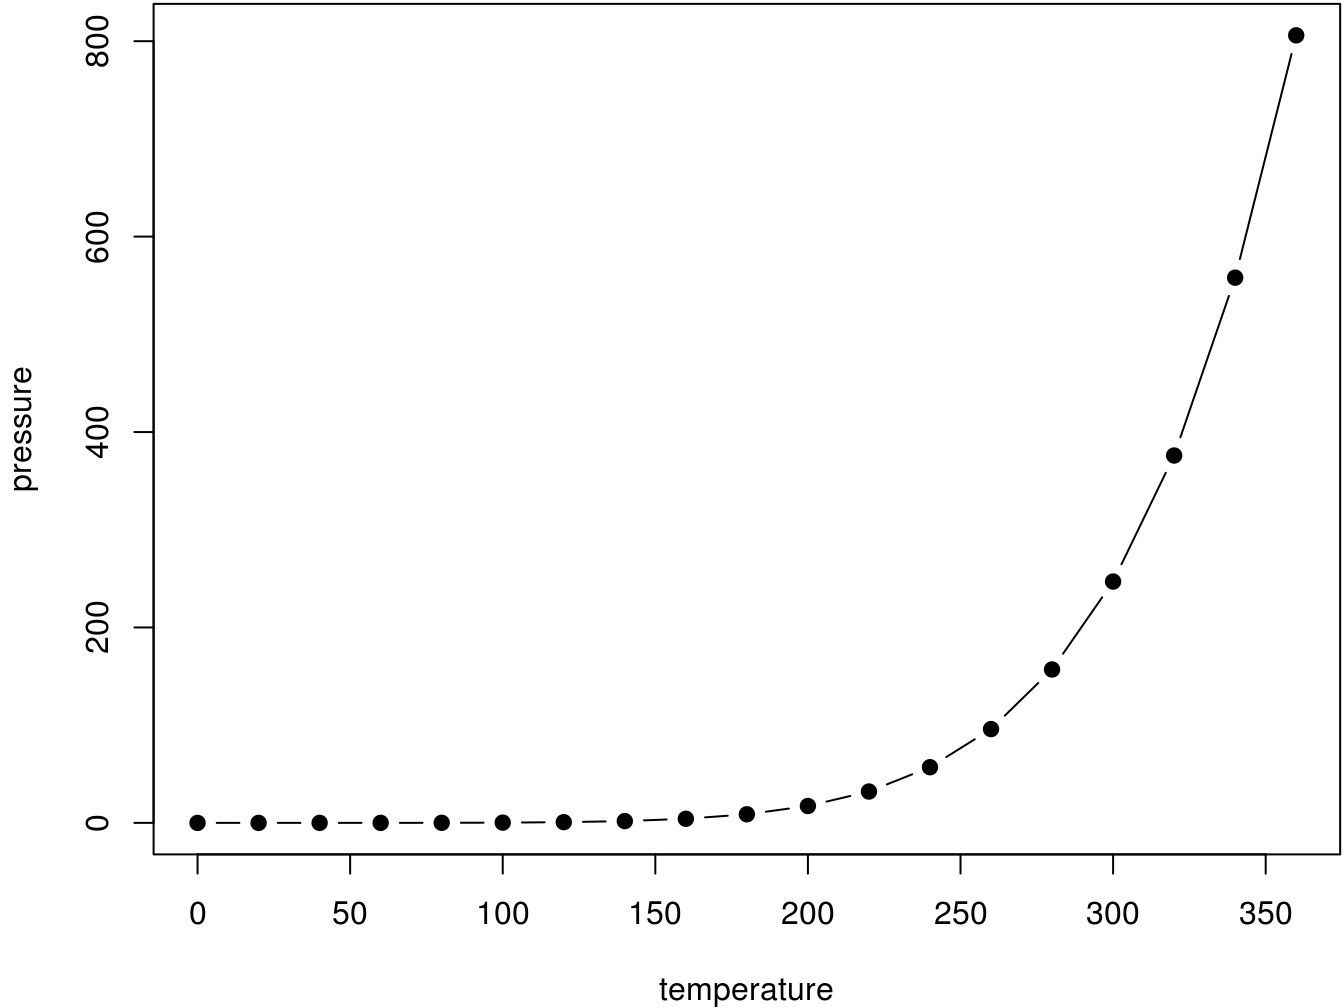
\includegraphics[width=0.8\linewidth]{01-intro_files/figure-latex/nice-fig-1} 

}

\caption{Here is a nice figure!}\label{fig:nice-fig}
\end{figure}

Reference a figure by its code chunk label with the \texttt{fig:} prefix, e.g., see Figure \ref{fig:nice-fig}. Similarly, you can reference tables generated from \texttt{knitr::kable()}, e.g., see Table \ref{tab:nice-tab}.

\begin{Shaded}
\begin{Highlighting}[]
\NormalTok{knitr}\OperatorTok{::}\KeywordTok{kable}\NormalTok{(}
  \KeywordTok{head}\NormalTok{(iris, }\DecValTok{20}\NormalTok{), }\DataTypeTok{caption =} \StringTok{\textquotesingle{}Here is a nice table!\textquotesingle{}}\NormalTok{,}
  \DataTypeTok{booktabs =} \OtherTok{TRUE}
\NormalTok{)}
\end{Highlighting}
\end{Shaded}

\begin{longtable}[]{@{}rrrrl@{}}
\caption{\label{tab:nice-tab}Here is a nice table!}\tabularnewline
\toprule
Sepal.Length & Sepal.Width & Petal.Length & Petal.Width & Species\tabularnewline
\midrule
\endfirsthead
\toprule
Sepal.Length & Sepal.Width & Petal.Length & Petal.Width & Species\tabularnewline
\midrule
\endhead
5.1 & 3.5 & 1.4 & 0.2 & setosa\tabularnewline
4.9 & 3.0 & 1.4 & 0.2 & setosa\tabularnewline
4.7 & 3.2 & 1.3 & 0.2 & setosa\tabularnewline
4.6 & 3.1 & 1.5 & 0.2 & setosa\tabularnewline
5.0 & 3.6 & 1.4 & 0.2 & setosa\tabularnewline
5.4 & 3.9 & 1.7 & 0.4 & setosa\tabularnewline
4.6 & 3.4 & 1.4 & 0.3 & setosa\tabularnewline
5.0 & 3.4 & 1.5 & 0.2 & setosa\tabularnewline
4.4 & 2.9 & 1.4 & 0.2 & setosa\tabularnewline
4.9 & 3.1 & 1.5 & 0.1 & setosa\tabularnewline
5.4 & 3.7 & 1.5 & 0.2 & setosa\tabularnewline
4.8 & 3.4 & 1.6 & 0.2 & setosa\tabularnewline
4.8 & 3.0 & 1.4 & 0.1 & setosa\tabularnewline
4.3 & 3.0 & 1.1 & 0.1 & setosa\tabularnewline
5.8 & 4.0 & 1.2 & 0.2 & setosa\tabularnewline
5.7 & 4.4 & 1.5 & 0.4 & setosa\tabularnewline
5.4 & 3.9 & 1.3 & 0.4 & setosa\tabularnewline
5.1 & 3.5 & 1.4 & 0.3 & setosa\tabularnewline
5.7 & 3.8 & 1.7 & 0.3 & setosa\tabularnewline
5.1 & 3.8 & 1.5 & 0.3 & setosa\tabularnewline
\bottomrule
\end{longtable}

You can write citations, too. For example, we are using the \textbf{bookdown} package (Xie \protect\hyperlink{ref-R-bookdown}{2020}) in this sample book, which was built on top of R Markdown and \textbf{knitr} (Xie \protect\hyperlink{ref-xie2015}{2015}).

\hypertarget{literature}{%
\chapter{Literature}\label{literature}}

Here is a review of existing methods.

\hypertarget{methods}{%
\chapter{Methods}\label{methods}}

We describe our methods in this chapter.

\hypertarget{applications}{%
\chapter{Applications}\label{applications}}

Some \emph{significant} applications are demonstrated in this chapter.

\hypertarget{example-one}{%
\section{Example one}\label{example-one}}

\hypertarget{example-two}{%
\section{Example two}\label{example-two}}

\hypertarget{final-words}{%
\chapter{Final Words}\label{final-words}}

We have finished a nice book.

\hypertarget{References}{%
\chapter*{参考文献}\label{References}}
\addcontentsline{toc}{chapter}{参考文献}

\hypertarget{refs}{}
\begin{cslreferences}
\leavevmode\hypertarget{ref-xie2015}{}%
Xie, Yihui. 2015. \emph{Dynamic Documents with R and Knitr}. 2nd ed. Boca Raton, Florida: Chapman; Hall/CRC. \url{http://yihui.name/knitr/}.

\leavevmode\hypertarget{ref-R-bookdown}{}%
---------. 2020. \emph{Bookdown: Authoring Books and Technical Documents with R Markdown}. \url{https://CRAN.R-project.org/package=bookdown}.
\end{cslreferences}

\end{document}
